\documentclass[10pt,conference]{IEEEtran}

\ifCLASSINFOpdf   
   \usepackage[pdftex]{graphicx}
   \graphicspath{{./Images/}}
   \DeclareGraphicsExtensions{.pdf,.jpeg,.png,.jpg}   
 \else   
   \usepackage[dvips]{graphicx}
\fi

\usepackage{caption}
\usepackage{fancyhdr}



\begin{document}

\title{ICS5114 Project\\Big Data Processing\\Speech Analytics On Live Streams}

\author{
    \IEEEauthorblockN{  Gabriel Sammut                  }
    \IEEEauthorblockA{  gabriel.sammut.13@um.edu.mt     }
\and
    \IEEEauthorblockN{  Nicholas Frendo                 }
    \IEEEauthorblockA{  nicholas.frendo.05@um.edu.mt    }
}

\IEEEspecialpapernotice{Academic Year 2018/2019}

\maketitle

%\thispagestyle{plain}
%\pagestyle{plain}
\pagestyle{fancy}
\fancyhf{}
\rhead{Speech Analytics on Live Streams}
\lhead{ICS5114 - Big Data Processing}
\rfoot{Page \thepage}


\section{Abstract}
The term ‘Big Data’ is often disguised under a range of shifting and evolving terms utilized to refer to the act of housing and processing of vast amounts of data. This endeavour however does not correlate only to the ever growing, large volumes of datasets, but is also used to refer to the rate of growth and the velocity at which it presents itself with. In addition, data of such vast speeds can also assume a myriad of forms, making it a challenge to effectively capture, process and produce useful information \cite{DataMiningWithBigData}. This scientific paper deals with issues presented by the velocity and variety aspects of Big Data, particularly to data of a live stream nature concerning video and text capture. This paper follows up to present possible scenarios and architectures to tackle the issues presented above and concludes with an evaluated benchmark of the proposed system.

\section{Introduction}
This scientific report attempts to encompass and document the work carried out to design and implement a high volume, multi-variety, distributed, data-processing system. The report will first address the presented challenges imposed by Big Data, as well as identify the two main objectives set out to achieve with the proposed system:
\begin{itemize}
    \item Variety
    \item Velocity
\end{itemize}
The report then follows up with a brief literature review with particular focus on literature focussed on resolving the proposed challenges. Eventually, the proposed design and architecture will be expanded upon, with particular highlights on the type of technologies utilized, and the reasons behind such choices. Eventually, the paper addresses two particular milestones, which serve to test the proposed system under load, particularly addressing content originating from various data streams. The paper concludes with an evaluation of the proposed system, detailing and contrasting the results of each milestone run and final thoughts with respect to problems encountered and the way they were tackled.
\\
A detailed mapping of all referenced figures throughout the report can be found in the appendix section, for the readers perusal.

\section{Problem Definition}
The following section addresses the many facets of the Big Data challenge, continuing with an explanation of the envisioned data processing system.

\subsection{Variety}
A congruent, well known challenge to the aspect of Big Data processing, results from data being produced from multiple sources, each source harnessing data of the same nature, but with different form and structure. In addition, the problem of variety extends further under varied guises, most predominantly; cases where data is being presented as varied textual, audio, video or cellular formats \cite{MgmtRevolution}. With data-producing giant firms serving unquantified amounts of data, the likes of which Facebook and Twitter are capable of generating on a daily basis, there is no common consensus, or agreeable format upon which dictates the transportation, consumption and storage of this data. Essentially, the problem of data variety falls upon the hands of the data consumer to tackle, requiring complex systems to cater for and build around the proposed problem. 

\subsection{Velocity}
Another active challenge of vast quantities of data, is the rate of incoming velocity at which the data presents itself with. The problem ties directly with the speed at which new data appears into a processing system. If the amount of data presented is not processed in a fast enough manner; that is, the incoming data generation rate is greater than the data processing and consumption rates, system backlogs and delays in data processing are inevitable. This is problematic, since such data would need to be accumulated, or otherwise is lost. In addition, this accumulation of data traffic can be problematic in itself, potentially overwhelming the system resources at hand if not catered to efficiently process and clear high velocity data \cite{MgmtRevolution}.
\\
Although the main problem lies within the remit of processing volumes of data at high speed, another potential pitfall relates to the over-provisioning of resources. It is common, that the rate of incoming data varies, depending on demand. This is difficult to plan around, requiring the data-processing system to be flexible with respect to utilized resources and incoming data. This poses a problem since any capable system must be able to plan around high intensive loads, whilst still ensuring that they operate efficiently without incurring additional costs in the case of low incoming data traffic.

\subsection{Dataset Selection}
One of the primary challenges of the proposed experiment was to locate a suitable source of high-traffic, rapid and varied streaming source of data. It was concluded that a pre-made dataset would be very hard, since all the following requirements needed to be met for the dataset to be valid for the proposed test scenario:
\begin{itemize}
\item Varied Data
    \begin{itemize}
        \item Varied Data Platforms
        \item Varied Data Content
    \end{itemize}
\item High Velocity Data
    \begin{itemize}
        \item Recorded Formats
        \item Streaming Formats
    \end{itemize}
\end{itemize}

The decision to test and evaluate the proposed system on a number of streaming platforms was taken, enabling the system to read from a constant fresh supply of new data, never ceasing in its data output. In addition, a number of varied streaming platforms were targeted, as well as attempting to process incoming data of both audio and textual formats. In particular, the following data sources were utilized for prototype testing, and/or eventual milestone evaluation:
\begin{itemize}
    \item Twitch.tv \cite{Twitch}
    \item YouTube \cite{YouTube}
    \item YouTube Live \cite{YouTubeLive}
    \item Daily Motion \cite{DailyMotion}
\end{itemize}

For the proposed milestone runs, YouTube and Twitch.tv were chosen for Milestone One and Milestone Two respectively. For both cases, both video and text data was captured and processed by the proposed system. 

\subsection{Aims and Objectives}
Therefore the aims of the proposed systems is two-fold; to tackle and present an efficient, scalable solution to the aforementioned two Vs of Big Data. The proposed architecture has been purposely modelled to handle and process rapid, incoming data streams, thus satisfying the Velocity aspect of big data. In addition, the presented solution also caters for the handling of different video and textual formats, from a number of varied platforms, thus fulfilling the Variety aspect of the presented problem.
\\
The proposed architecture would therefore record all incoming information, both textual and video. In the case of video data streams, an additional transcription step is required in order to convert the audio channel into its textual representation. Subsequently, the resulting data is stored in a graphical network of users, representing viewers and streamers, in relation to word utterance and count. The end result of such a system is expected to behold a number of online users, coming from various platforms, in relation to their respective words uttered, in the form of a graph network for metric evaluation.

\section{Background and Related Systems}
The aspect of handling rapid, varied and large quantities of incoming data is already coined as a subset of Big Data. Through the widespread use of internet-based applications, huge quantities and varieties of data are churned at unprecedented rates, making it a challenge to harness information from the torrents of incoming data \cite{BigDataYahoo, VideoCloudPlatform}. It is well established that for any proposed architecture to tackle the challenges posed by big data, it must conform with the following standards \cite{VideoCloudPlatform, DeepIntelligenceFramework}:
\begin{itemize}
    \item \textit{Performance,} speed with which to process data as fast as possible.
    \item \textit{Scalability,} requiring the architecture to be flexible enough to grow on demand.
    \item \textit{Fault Tolerance,} ensuring that enough redundancy is present to maintain optimum up-time rates, therefore reducing data loss.
\end{itemize}

These standards play well into the CAP Theorem perspective \cite{CAPTheorem}, imposing further challenges to maintain an architecture capable of fulfilling all three subsets.
\\
A number of Big Data oriented frameworks are well established in the field, with processing platforms such as the batch processing Hadoop toolset having achieved great success in this particular domain \cite{VideoCloudPlatform, Hadoop}. However, the MapReduce paradigm leaves much to be desired with respect to the challenges posed by high velocity streams, due to it’s batch-like nature. This limitation is further emphasized for time-sensitive data stream processing, particularly that of real-time video and audio data capture.
\\
Particular notable mentions include Yahoo!S4, coined as ‘a general-purpose, distributed, scalable, fault-tolerant, pluggable platform’, created for the purpose of unbounded data stream processing \cite{VideoCloudPlatform}. Apache Kafka fits well in this bracket, allowing ceaseless interaction between distributed, communicating modules, allowing them to operate under a publish-subscribe design pattern \cite{Kafka}. Another component of the Apache toolset is the Spark framework \cite{UnifiedEngine}, promising fast and stream capable performance, as well as offering seamless integration for machine learning components.
\\
It is however Apache Storm which fully dedicates itself to the challenge presented by velocity of incoming data \cite{Storm}. Compared to the well established Hadoop MapReduce architecture, Storm makes it easy to reliably integrate with unbounded streams of data, whilst still offering the capacity for large data volumes. For the variety aspect of Big Data, Storm tackles this through the use of stream repartitioning \cite{VideoCloudPlatform}, making it a handy tool set in tackling the three major Vs \cite{DeepIntelligenceFramework, CAPTheorem}.

\section{Architecture - Big Data Design}
The following section incorporates design decisions concerning the proposed architecture. It then proceeds by taking a closer look into each component of the proposed architecture in further detail.

\subsection{Overview}
The presented solution is essentially a distributed system, operating over a cloud based network, composed of at least four concurrent running nodes. Each node forms an essential part to what is essentially a pipelined process, with each node being fed data, processes the data and passes it onto the subsequent processing node. The following key, architectural terms will be referenced throughout the remainder of this report:
\begin{itemize}
    \item \textbf{Producer} - The producer script is custom made written logic utilized to acquire data from a data source, download it locally onto the machine running the process and offload it onto a Kafka \cite{Kafka} broker. The script is capable of handling pre-recorded data similar to that of on-demand YouTube video content, as well as capable of recording streaming, live footage feed.

    \item \textbf{Apache Kafka} - Kafka is a distributed streaming platform, capable of publishing and subscribing to streams of records. The prime concept behind Kafka is loosely modelled on the produce-consume methodology. The architecture offers support for the storage of records in a fault-tolerant and durable manner, capable of streaming records simultaneously depending on the demand of the incoming data streams \cite{Kafka}.

    \item \textbf{Apache Storm} - For the reliable processing of unbounded streams, Apache Storm was the ideal choice \cite{Storm}. Utilizing the Kafka-Spout component, the Storm topology was fed data directly from the Kafka broker. The utility of storm enabled the ease of scaling processing dependent on demand, allowing the storm topology to parallelize each spout/bolt internally for greater processing throughput, as well as offering the capability of distributing work undergoing in the topology over a distributed network of storm workers. Storm also offers a level of fault tolerance, however this configuration was not enforced heavily in the proposed architecture, since all storm components were placed on a single operating machine.

    \item \textbf{Neo4j Graph Platform} - The prime goal of the proposed system is to capture and model words uttered by online users, be it through audio or textual utterance. The Neo4j graph database, being a high performance graph store whilst retaining the robustness of a mature database \cite{Neo4j}, was the perfect choice for such a data capture scenario. With heavy focus on relation modelling, insertion and retrieval of related nodes made Neo4j particularly suited for this task. In addition, the innate graph representation enhances the speed at which related data can be retrieved, especially so for larger volumes as the database grows larger. This is a stark contrast to generic relational databases, in which data relationships become complex to model and retrieve using conventional table join methods.

    \item \textbf{Google Cloud Platform} - For video decoding and speech to text functionality, the Cloud Speech-to-text API was utilized, allowing the proposed system to upload video segments via the API, decode them, and extract respective decoded video clippings back into the system \cite{GoogleSpeech}. Decoding of video to text is done in parallel to the actual submission of the streaming object through Kafka, and Storm.
\end{itemize}

The proposed architecture is capable of handling pre-recorded online data, as well as handling real-time streams. The following diagrams provide a holistic view of the proposed system, in light of both recording and streaming modes.

\begin{figure}
  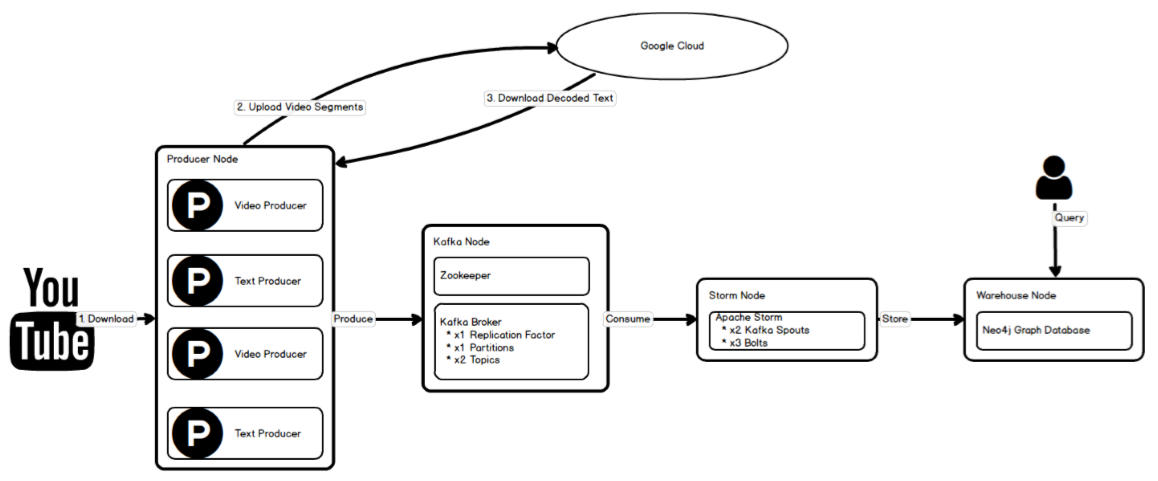
\includegraphics[width=\linewidth]{HolisticOverviewRecording.png}
  \caption                          {Holistic Overview - Recording}
  \label                            {fig:HolisticOverviewRecording}
\end{figure}

\begin{figure}
  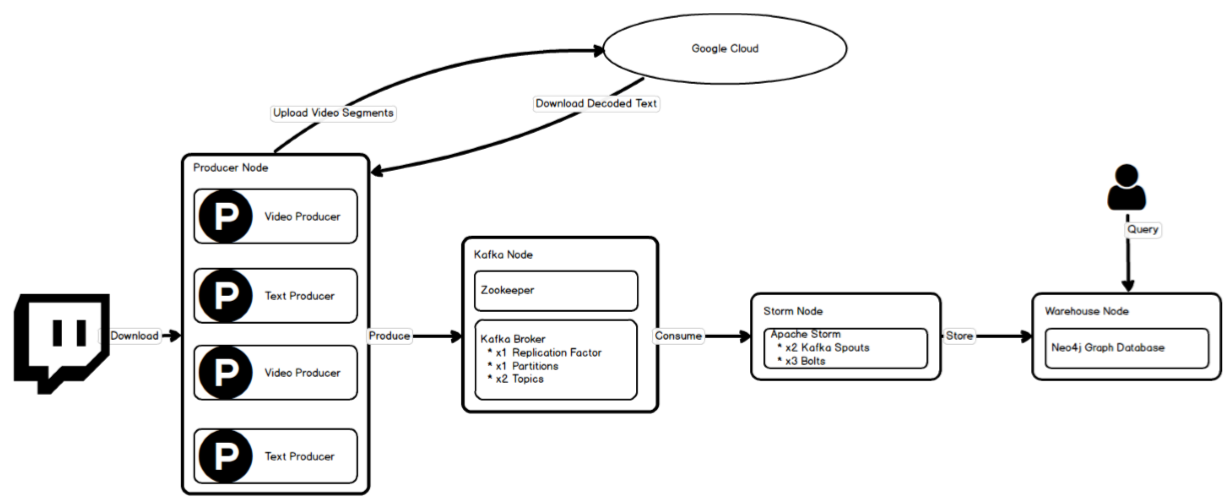
\includegraphics[width=\linewidth]{HolisticOverviewStreaming.png}
  \caption                          {Holistic Overview - Streaming}
  \label                            {fig:HolisticOverviewStreaming}
\end{figure}

\subsection{Producer}
The producer is tasked to interface with the data source by and downloading the data locally and submitting it onto the pipeline by offloading data into the Kafka broker. The producer script is written in a way to handle various data formats, both textual and video formats. For text capturing, the YouTube API \cite{YouTubeAPI} was used to interface with and capture channel comments, by first downloading each respective channel comment thread, followed by each respective comment itself and eventually submitting all textual comments onto a Kafka-topic reserved for text handling. In addition, a second form of text capture was added to the producer, allowing the current functionality to interface with real time live chats produced from Twitch.tv streams, through the use of IRC \cite{TwitchChatBot}.

\begin{figure}
  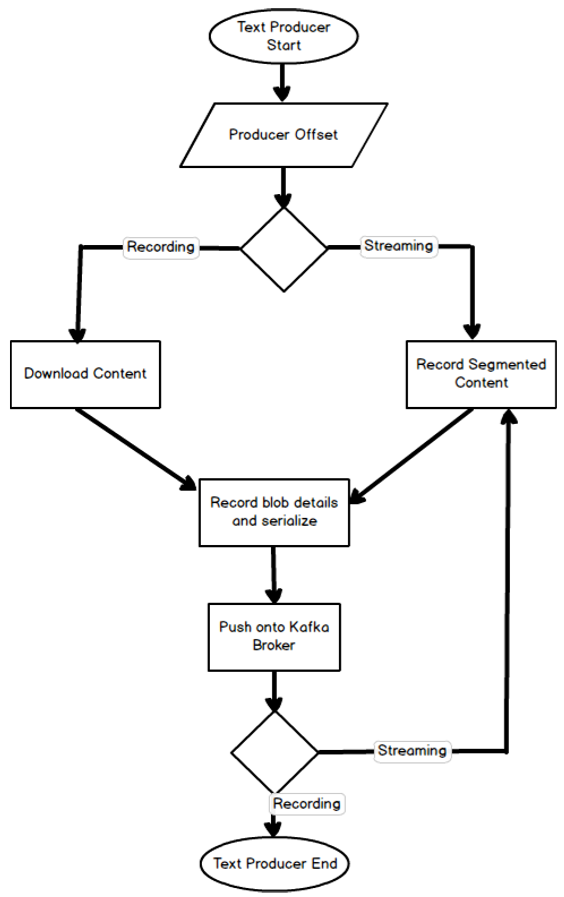
\includegraphics[width=\linewidth]{ProducerTextFlow.png}
  \caption                          {Text Producer Processing Flow}
  \label                            {fig:ProducerTextFlow}
\end{figure}

\begin{figure}
  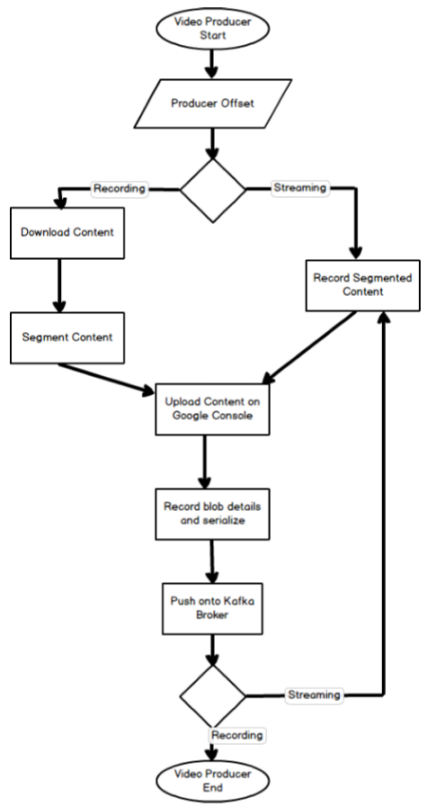
\includegraphics[width=\linewidth]{ProducerVideoFlow.png}
  \caption                          {Video Producer Processing Flow}
  \label                            {fig:ProducerVideoFlow}
\end{figure}

For video capture, a set of wrapper scripts were written into the producer. For pre-recorded video extraction, the pythonic library ‘pytube’ \cite{PyTube} was used, allowing the producer to download any number of YouTube video footage, segment it locally through usage of ffmpeg \cite{Ffmpeg} into snippets of preconfigured time (preconfigured to thirty seconds by default) and upload each segmented clip onto the Google Cloud Platform. The endpoint of the upload video blob storage is annotated along with several other information criteria and submitted onto the Kafka broker.
\\
For real-time video capture, the streaming tool ‘Streamlink’ \cite{Streamlink} was used through the automated use of the producer. The tool allows real-time stream capturing of video data, particularly tried and tested on Twitch.tv and YouTube-Live. Similar to the pre-recording video logic, Streamlink is used to record live-streams for thirty seconds straight. The resulting segmented clip is uploaded to Google Cloud Platform and submitting the respective uploaded video blob storage URL through Kafka.

\subsection{Kafka}
The usage of Apache Kafka allows the graceful interaction between Producer and Storm components, allowing both Producer and Storm to act as the ‘producer’ and ‘consumer’ respectively. For the purposes of the proposed system, Kafka was limited to a total of two partitions with the following settings:
\\
\\
\\
Kafka Video Topic
\begin{itemize}
    \item N. Partitions: 1
    \item Replication Factor: 1
\end{itemize}
Kafka Text Topic

\begin{itemize}
    \item N. Partitions: 1
    \item Replication Factor: 1
\end{itemize}

\subsection{Storm}
The storm toolset was utilized through a pythonic wrapper called ‘Streamparse’ \cite{Streamparse}, allowing the topology itself and each Storm component to be written in native Python. The topology structure was composed of the following components:

\begin{table}[h]
    \centering
    \begin{tabular}{|c|c|c|}
        \hline
        Component&Component&Parallel    \\
        Type&Name&Degree                \\ \hline
        Spout&video\_recording\_spout&1 \\ \hline
        Spout&text\_recording\_spout&1  \\ \hline
        Bolt&video\_decoder\_bolt&4     \\ \hline
        Bolt&text\_decoder\_bolt&1      \\ \hline
        Bolt&graph\_writer&2            \\ \hline
    \end{tabular}
    \captionof{table}{Storm Topology}
    \label{tab:StormTopology}
\end{table}

Each of the two spouts utilize the Kafka-Spout Implementations, serving as a consumer to the Apache Kafka architecture, each spout subscribed to its respective kafka topic. Once subscribed, each kafka spout actively listens for incoming data on the kafka partition, at which point data is passed down the topology onto the ‘video\_recording\_bolt’ or ‘text\_recording\_bolt’, for processed video and text data respectively. It is here that both bolts carries out a number of text processing techniques onto the oncoming text, including:
\begin{itemize}
    \item Stop Word Removal
    \item Stemming of Words
    \item Special Character/Symbol Removal
    \item Single Character Removal
\end{itemize}

Lemmatizing of incoming data was considered, but eventually left out, with testing results indicating that particular words were being transformed into undesirable pronunciations of the original word.
\\
The ‘video\_decoder\_bolt’, in addition to the aforementioned text processing is required to connect to the Google Cloud Platform via usage of the Google Cloud Platform API, by which point would have already been decoded by the previously uploaded video from the producer node. The video\_decoder\_bolt therefore requests the blob URL storage passed through the pipeline, retrieves the decoded text, processes it locally and submits it down the pipeline.
\\
The ‘graph\_writer’ bolt actively listens to incoming data traffic from the the ‘video\_decoder\_bolt’ and ‘text\_decoder\_bolt’, saving all textual data to the graph storage node.

\begin{figure}[h]
  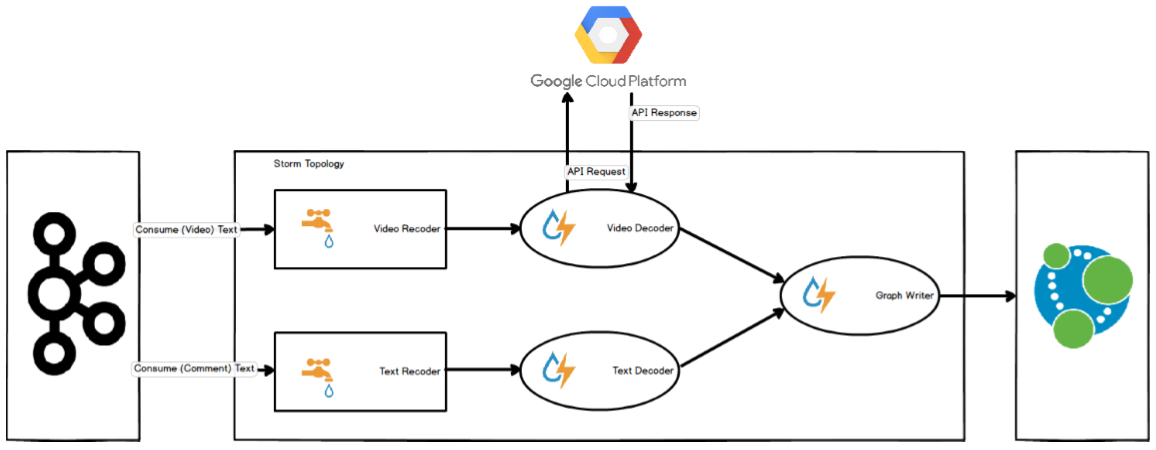
\includegraphics[width=\linewidth]{StormTopology.png}
  \caption                          {Storm Topology}
  \label                            {fig:StormTopology}
\end{figure}

\subsection{Neo4j}
The graph database serves as a suitable endpoint for the pipeline, which receives and stores all textual data in the form of a graph. The graph serves to model received data as follows: \\
Nodes:
\begin{itemize}
    \item Streamer
    \item Viewer
    \item Genre
    \item Word
    \item Platform
\end{itemize}

\begin{table}[h]
    \centering
    \begin{tabular}{|c|c|c|}
        \hline
        \textbf{Node 1}&\textbf{Relationship}&\textbf{Node 2}   \\ \hline
        Streamer&Utters&Word                                    \\ \hline
        Viewer&Comments&Word                                    \\ \hline
        Word&Features&Genre                                     \\ \hline
        Viewer&Follows&Genre                                    \\ \hline
        Streamer&Partakes&Genre                                 \\ \hline
        Viewer&Subscribes&Streamer                              \\ \hline
        Streamer&Uses&Platform                                  \\ \hline
    \end{tabular}
    \captionof{table}{Storm Topology}
    \label{tab:GraphRelationships}
\end{table}

For graph edges of type ‘Utters’ and ‘Comments’, each respective word utterance is counted per streamer and viewer respectively. In addition, those nodes of type ‘Word’ contain an additional boolean flag variable called ‘foul\_flag’, which denotes whether the word is registered as foul language, as denoted by a pre-recorded foul word corpus [24]. Only foul words of an English syntax are tracked.

\begin{figure}[h]
    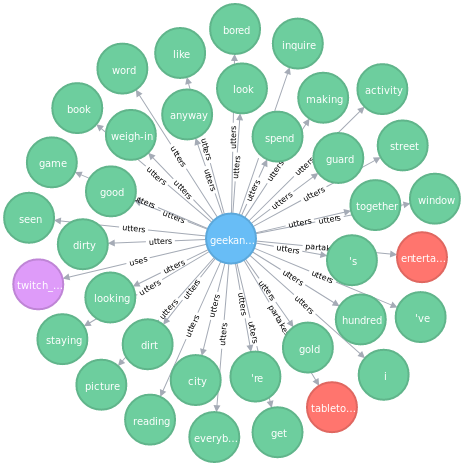
\includegraphics[width=\linewidth]{GraphTopology.png}
    \captionsetup                     {justification=centering}
    \caption                          {Graph Topology\\Blue Node: Streaming Channel\\
                                       Green Node: Word Utterance\\Red Node: Attributed Genre\\Purple Node: Streaming Platform}
    \label                            {fig:GraphTopology}
\end{figure}

\section{System Setup}
The Speech Analytics system was compartmentalized into individual modules, forming the entire end-to-end system pipeline, as previously discussed. Whilst designing a strategy of bringing all the modules together, priority was given to the following aspects:
\begin{itemize}
    \item \textit{Costs}            \\ Maximizing the available cloud computing resources.
    \item \textit{Test environment} \\ A convenient environment that mimics the cloud setup for system debugging purposes.
    \item \textit{Time}             \\ Minimizing the development to deployment cycle time.
                                    \\ Automating the deployment procedure.
\end{itemize}

\subsection{System Components}
The entire pipeline was broken down into four unique modules, namely Producer, Kafka, Storm and Neo4J. All the individual modules were contained into separate Docker images, as depicted below:

\begin{figure}[h]
    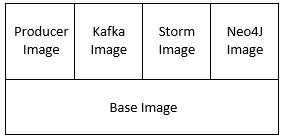
\includegraphics[width=\linewidth]{DockerImageHierarchy.png}
    \captionsetup                     {justification=centering}
    \caption                          {Docker Image Hierarchy}
    \label                            {fig:DockerImageHierarchy}
\end{figure}

All the shared software components and python packages were included into the base Docker image. On top of that, additional Docker images were built, each specific to a given Speech Analytics system module. This approach made the Docker image construction flexible, especially during the initial development stages were the software components and python packages were still not fully established. Once all Docker images were constructed, the images were appropriately tagged and uploaded to DockerHub \cite{DockerHub}.

\subsection{System Deployment Automation}
System deployment and execution was done on two separate environments. A test environment was set up through VirtualBox \cite{VirtualBox} such that it mimics the actual live environment. The live environment was employed on the Microsoft Azure cloud computing \cite{Azure} platform.
\\
A utility tool was developed that handles the entire system automation aspect. This was achieved through Bash scripts that make use of tools such as Docker, Docker-Machine and Nmap. This tool abstracted away the details between the local test environment and the remote Azure platform, thus commands issues were seamlessly executed on either one of the environments. The below utility features were implemented:
\begin{itemize}
    \item \textit{VM creation and deletion} \\
    VM quantities and resource specifications were specified in an external configuration file. \\
    As part of the VM creation process, the appropriate Docker image was pulled from the DockerHub repository into the newly created machine.
    \item \textit{VM start and stop}
    \item \textit{Docker container start and stop} \\
    The Docker container start-up followed a specific start-up sequence, based upon the inherent dependency between the respective Docker containers. \\
    As part of the Docker container start-up, the python code was pulled from the GitHub repository. This made it convenient, since no changes were required following any changes to the source code. \\
    Docker containers were not persisted after being unloaded from memory, thus eliminating any container management requirements. \\
    In the specific case of the Neo4J container, a drive was mapped on the host file system in order to persist the generated data.
    \item \textit{Docker container telemetry} \\
    Docker statistics, including CPU, memory and bandwidth usage. \\
    Docker logging, useful for debugging purposes.
\end{itemize}

\section{Milestones}
To benchmark and evaluate the proposed system, a total of two milestones were planned. Both milestones served as checkpoints which would test the system under different scenarios and conditions, allowing for a more robust evaluation of the implemented infrastructure.

\subsection{Milestone One}
The first of the two proposed milestones aimed at smoke testing the proposed pipeline, ensuring that all basic and detrimental functionality is working well under limited volumes. The test was aimed particularly at pre-recorded footage and pre-recorded text, particularly from YouTube sources. This makes the test more controllable in terms of data being pumped into the system. With limited, yet sufficient volumes being inserted down the pipeline, ensures that almost all aspects of the architecture has been tested.

\subsection{Milestone Two}
The second proposed milestone is intended to expose the proposed architecture to real-time streaming data, so as to evaluate and gauge the effectiveness of the system under high velocity streams. In addition, the objective here is also to stress-test the pipeline as follows:
\begin{itemize}
    \item Stress-test the system with double or more data than the original milestone.
    \item Stress-test the system by leaving the pipeline running for double the time it took for milestone one.
\end{itemize}

\section{Evaluation}
System evaluation and overall performance was gauged and benchmarked on each of the proposed milestones. Each of the installed architecture components were monitored individually to achieve insight as to their granular behaviour. In addition, several graph visualizations were created to visualize the underlying data, as well as provide a series of data analytics techniques.

\subsection{Milestone One - Results and Interpretation}
The first of the aforementioned milestones tested the proposed architecture on pre-recorded data specifically on the following YouTube content \cite{YouTubeLastWeekTonightChannel}. The following approximate timings were recorded as follows:

\begin{table}[h]
    \centering
    \begin{tabular}{|c|c|c|c|}
        \hline
        \textbf{Entity}&\textbf{Process}&\textbf{Process}&\textbf{Total}    \\
        &\textbf{Start}&\textbf{End}&\textbf{Time}                          \\ \hline
        Producer2&05:37:44&10:37:00&05:00:00                                \\
        (Video)&&&                                                          \\ \hline
        Producer3&05:37:44&13:00:00&07:23:00                                \\
        (Text)&&&                                                           \\ \hline
        Producer4&05:37:44&10:37:00&05:00:00                                \\
        (Video)&&&                                                          \\ \hline
        Producer5&05:37:44&13:00:00&07:23:00                                \\
        (Text)&&&                                                           \\ \hline
        Kafka&05:37:44&13:00:00&07:23:00                                    \\ \hline
        Storm&05:37:44&13:00:00&07:23:00                                    \\ \hline
        Neo4j&05:37:44&13:00:00&07:23:00                                    \\ \hline
    \end{tabular}
    \captionof{table}{Milestone 1 Producer Timings}
    \label{tab:Milestone1Timings}
\end{table}

During the above mentioned time window, performance metrics were extracted and visualized. These metrics allow a clearer insight with respect to individual component performance, including CPU, Main Memory and Physical I/O Usage:

\begin{figure}[h]
    \centering
    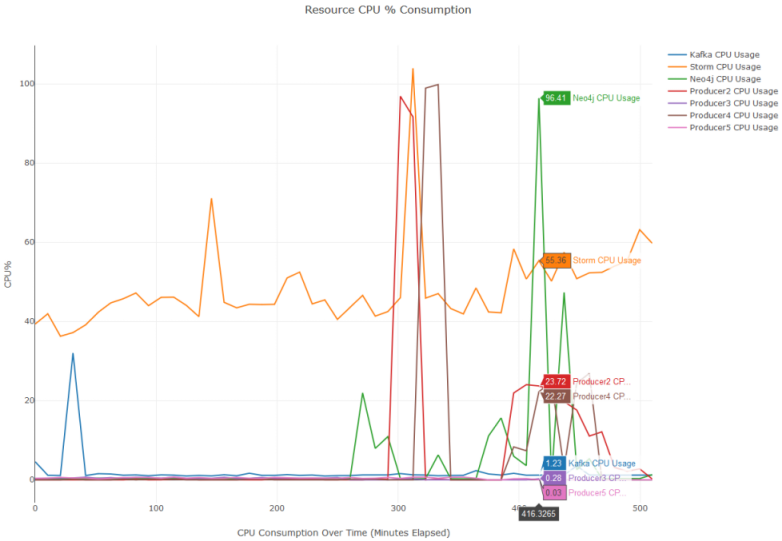
\includegraphics[height=3.5cm,keepaspectratio]{Milestone1CpuUsage.png}
    \captionsetup                                 {justification=centering}
    \caption                                      {Milestone 1 - Cpu Usage}
    \label                                        {fig:Milestone1CpuUsage}
\end{figure}

\begin{figure}[h]
    \centering
    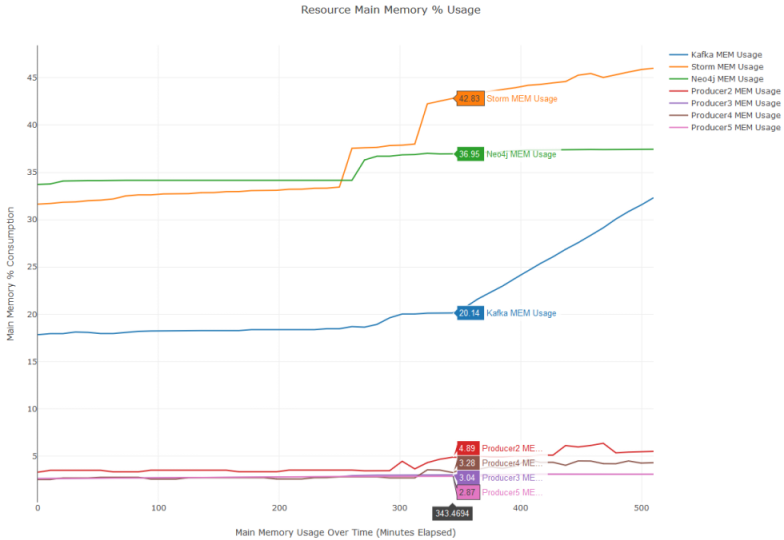
\includegraphics[height=3.5cm,keepaspectratio]{Milestone1MemoryUsage.png}
    \captionsetup                                 {justification=centering}
    \caption                                      {Milestone 1 - Memory Usage}
    \label                                        {fig:Milestone1MemoryUsage}
\end{figure}

\begin{figure}[h]
    \centering
    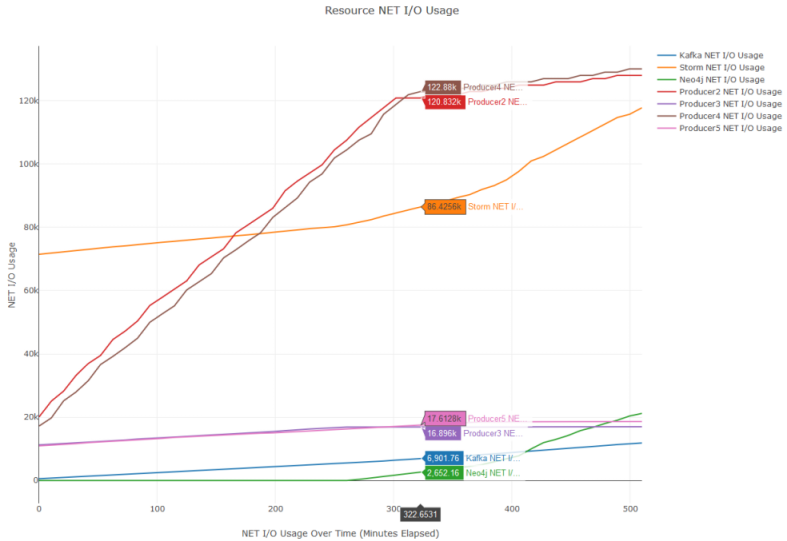
\includegraphics[height=3.5cm,keepaspectratio]{Milestone1NetUsage.png}
    \captionsetup                                 {justification=centering}
    \caption                                      {Milestone 1 - Network I/O Usage}
    \label                                        {fig:Milestone1NetUsage}
\end{figure}

As an interactive visualization capable of monitoring data dynamics, an interactive graph model was established, based upon the generated graph structure from milestone one. The graph allows the user the possibility of navigating each respective word, streamer relationship. Each graph edge denotes the total number of word utterances from the respective viewer and/or streamer.

\begin{figure}[h]
    \centering
    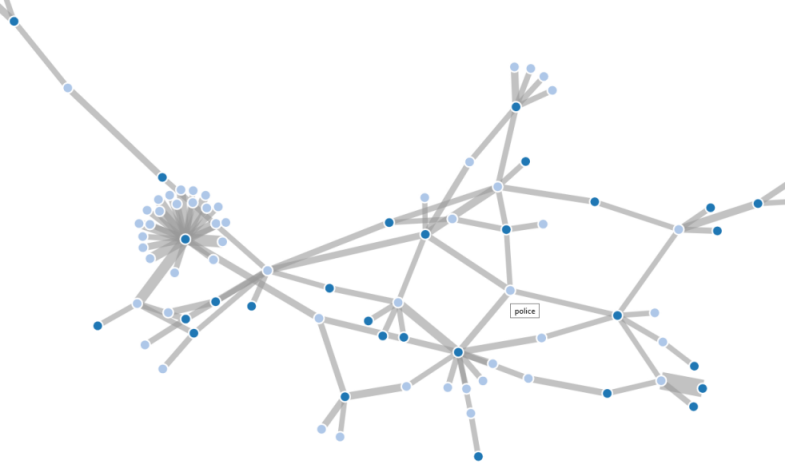
\includegraphics[height=3.5cm,keepaspectratio]{InteractiveViewer.png}
    \captionsetup                                 {justification=centering}
    \caption                                      {Interactive Viewer/Streamer Word Utterance}
    \label                                        {fig:InteractiveViewer}
\end{figure}

Based upon the established timings, overall performance and system behaviour, it was decided that the pipeline operated as expected during the entirety of milestone one. Each of the distributed components and respective VMs were not exhausted by the volume of the input data streams, with the entire system behaving in a stable manner.

\subsection{Milestone Two - Results and Interpretation}
The second milestone was focussed on stress testing the system so as to ensure optimum quality during real-time input data streaming, over a longer period of time. The experiment ran for a total of nineteen hours, with eight constant input streams being channelled through the pipeline. The following performance metrics were recorded as follows, particularly for Kafka, Storm and the Neo4j environments:

\begin{figure}[h]
    \centering
    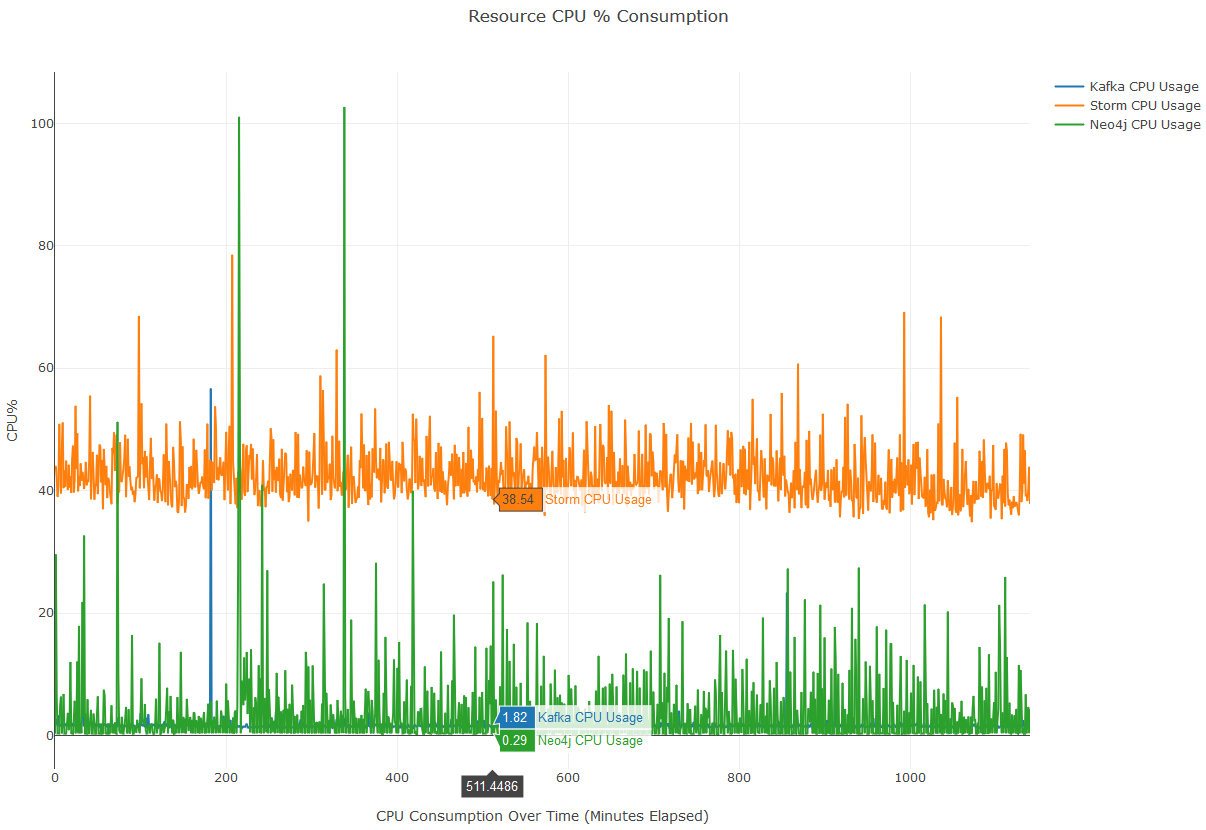
\includegraphics[height=3.5cm,keepaspectratio]{Milestone2CpuUsage.png}
    \captionsetup                                 {justification=centering}
    \caption                                      {Milestone 2 - Cpu Usage}
    \label                                        {fig:Milestone2CpuUsage}
\end{figure}

\clearpage

\begin{figure}[h]
    \centering
    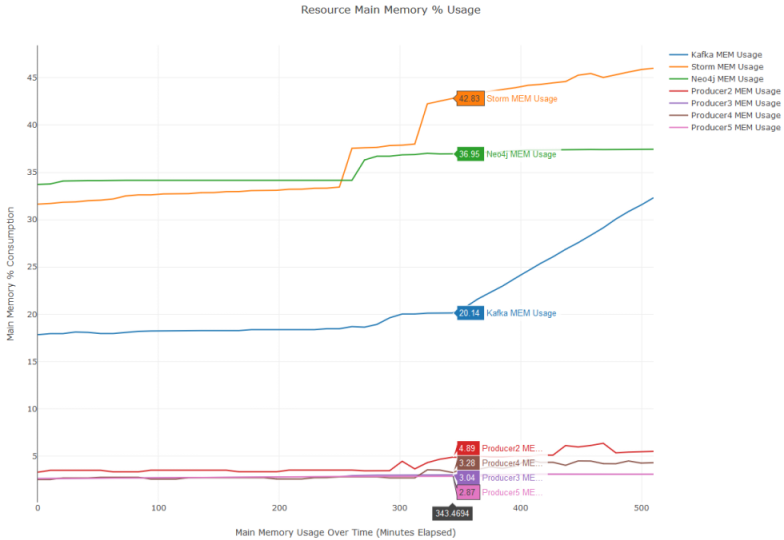
\includegraphics[height=3.5cm,keepaspectratio]{Milestone1MemoryUsage.png}
    \captionsetup                                 {justification=centering}
    \caption                                      {Milestone 1 - Memory Usage}
    \label                                        {fig:Milestone1MemoryUsage}
\end{figure}

\begin{figure}[h]
    \centering
    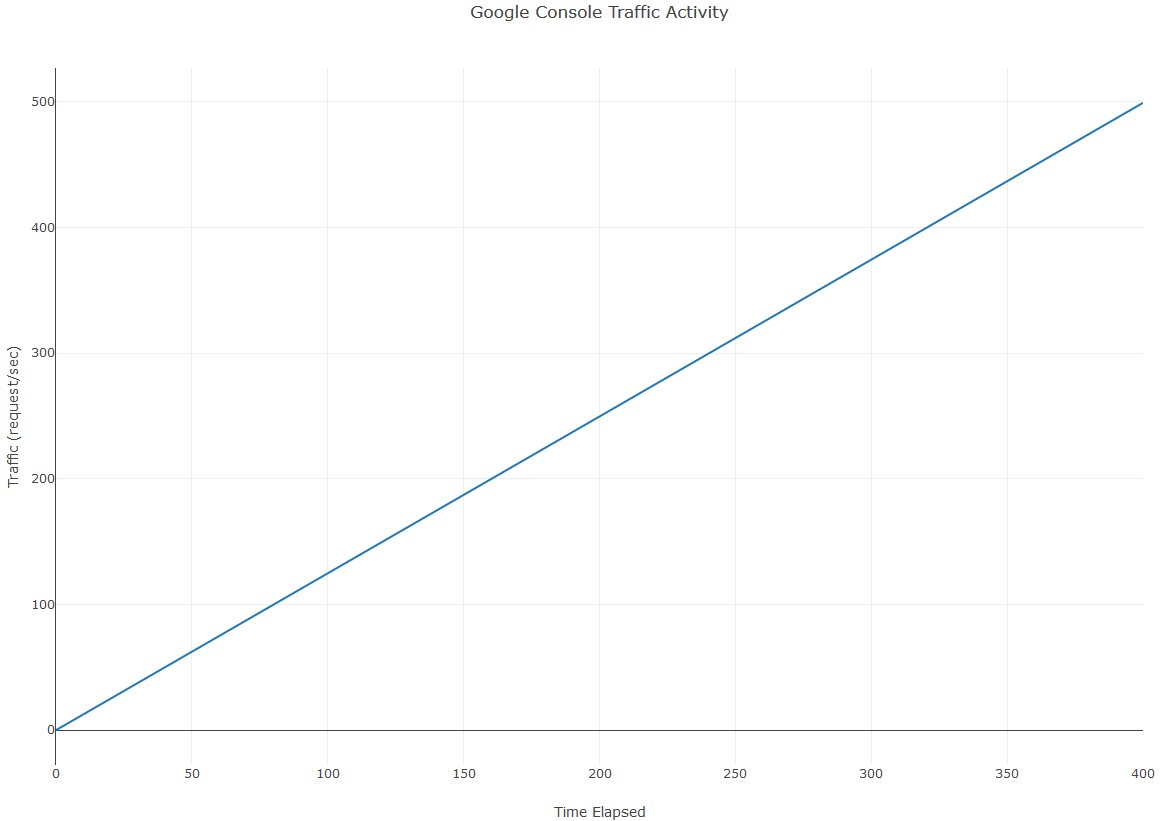
\includegraphics[height=3.5cm,keepaspectratio]{Milestone2NetUsage.png}
    \captionsetup                                 {justification=centering}
    \caption                                      {Milestone 2 - Network I/O Usage}
    \label                                        {fig:Milestone2NetUsage}
\end{figure}

The above figures indicate a stable, gradual performance of the tested pipeline components. Of particular notice is the resource hungry presence of Storm, when compared to the Kafka and Neo4j entities. Statistics for each respective producer were also extracted, as follows:

\begin{figure}[h]
    \centering
    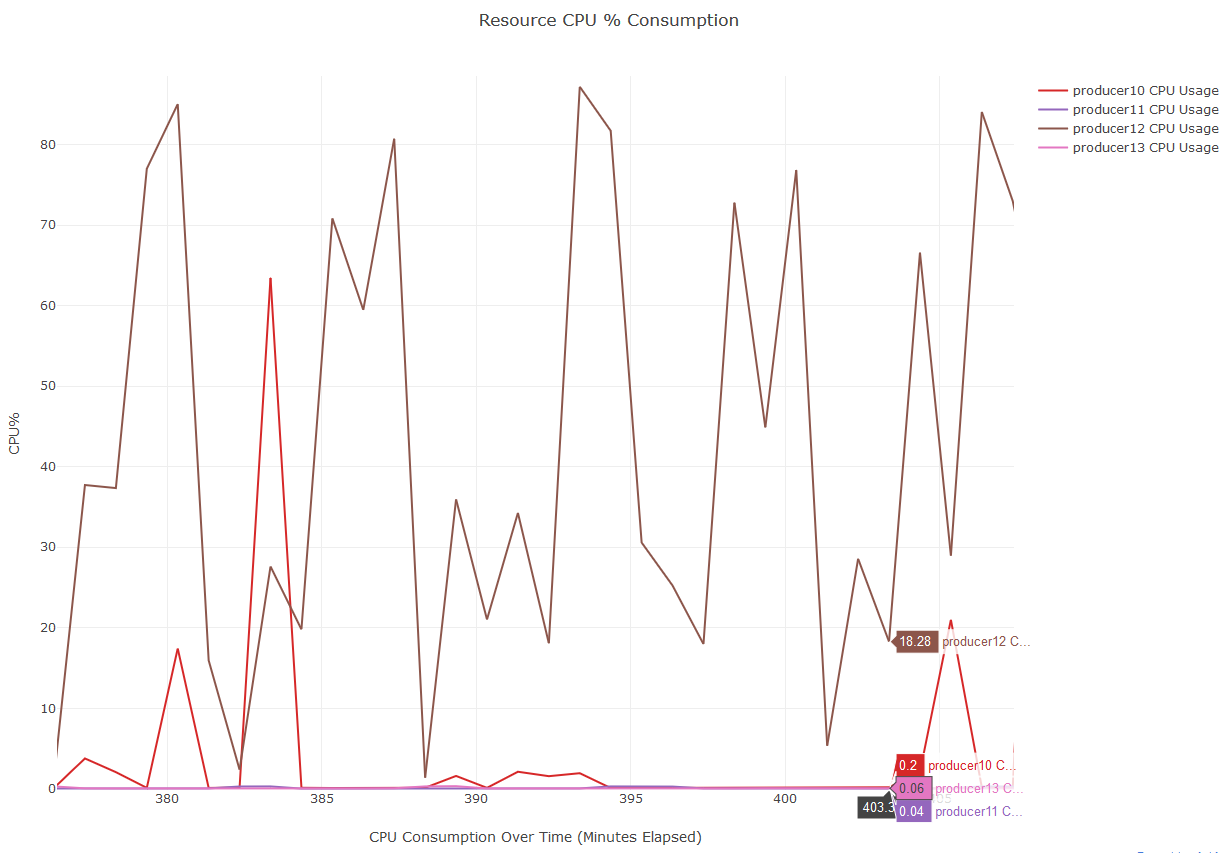
\includegraphics[height=3.5cm,keepaspectratio]{Milestone2ProducerCPU.png}
    \captionsetup                                 {justification=centering}
    \caption                                      {Milestone 2 - Producer CPU Usage}
    \label                                        {fig:Milestone2ProducerCPU}
\end{figure}

The above metrics suggest a particular strain on the producer node, particularly so those responsible for processing video. CPU usage was visible to have been operating at over 80\% at particular times, suggesting a potential hardware bottleneck, which can be tackled by scaling video processing nodes in a vertical manner.

\subsection{Additional Requirements}
The following section is dedicated particularly on the following three aspects, all of which were directed upon the graph store for milestone two:
\begin{itemize}
    \item Data Analytics
    \item Data Dynamics
    \item Data Visualizations
\end{itemize}

\begin{figure}[h]
    \centering
    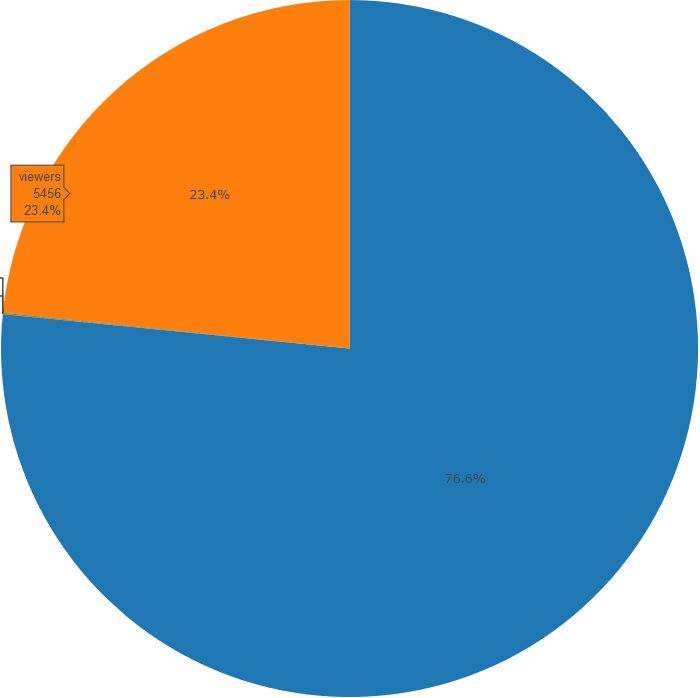
\includegraphics[height=3.5cm,keepaspectratio]{NodeQuantityRatio.png}
    \captionsetup                                 {justification=centering}
    \caption                                      {Node Quantity Ratio}
    \label                                        {fig:NodeQuantityRatio}
\end{figure}

\begin{table}[h]
    \centering
    \begin{tabular}{|c|c|c|}
        \hline
        \textbf{Node Type}&\textbf{Node Count}&\textbf{Node [\%]}   \\ \hline
        Word&17,880&76.600\%                                        \\ \hline
        Viewer&5456&23.400\%                                        \\ \hline
        Genre&9&0.038\%                                             \\ \hline
        Streamer&4&0.017\%                                          \\ \hline
        Platform&1&0.004\%                                          \\ \hline


    \end{tabular}
    \captionof{table}{Milestone 2 Node Counts}
    \label{tab:Milestone2NodeCounts}
\end{table}

\begin{figure}[h]
    \centering
    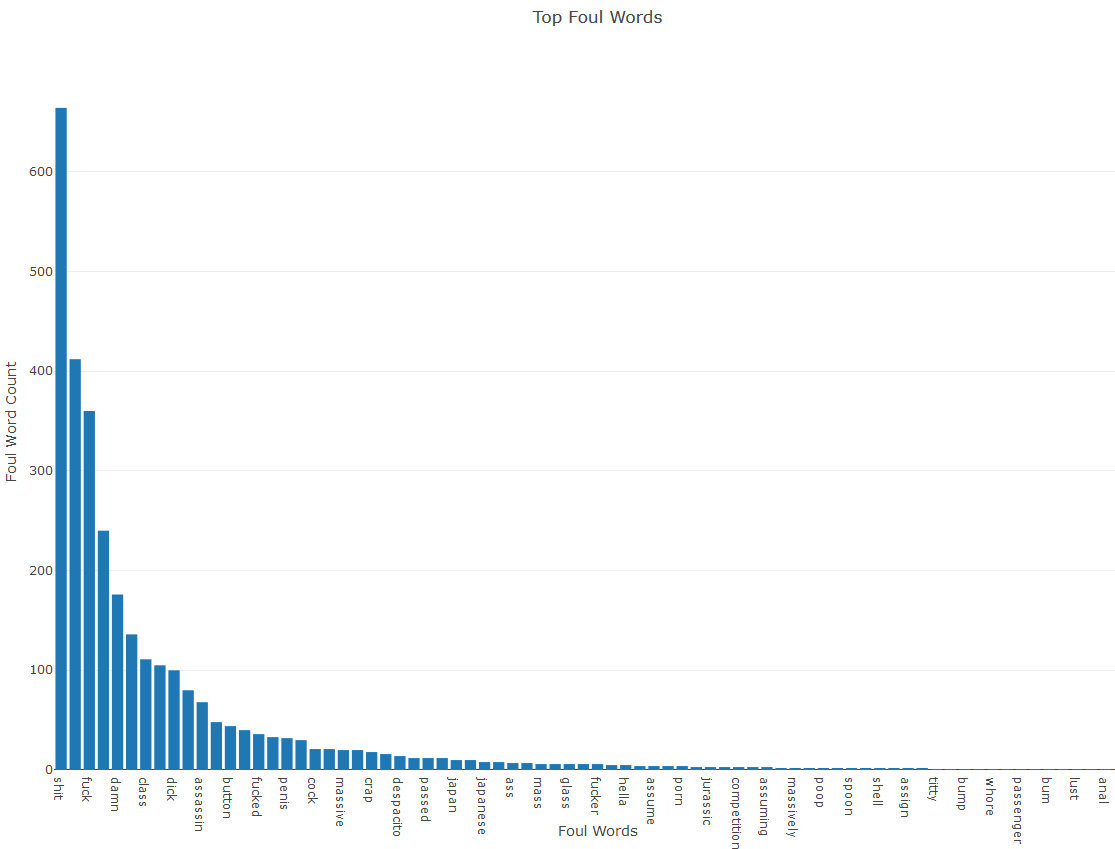
\includegraphics[height=4cm,keepaspectratio]{FoulWordUsage.png}
    \captionsetup                               {justification=centering}
    \caption                                    {Foul Word Usage, Ranked By Highest Occurrence}
    \label                                      {fig:FoulWordUsage}
\end{figure}

\begin{figure}[h]
    \centering
    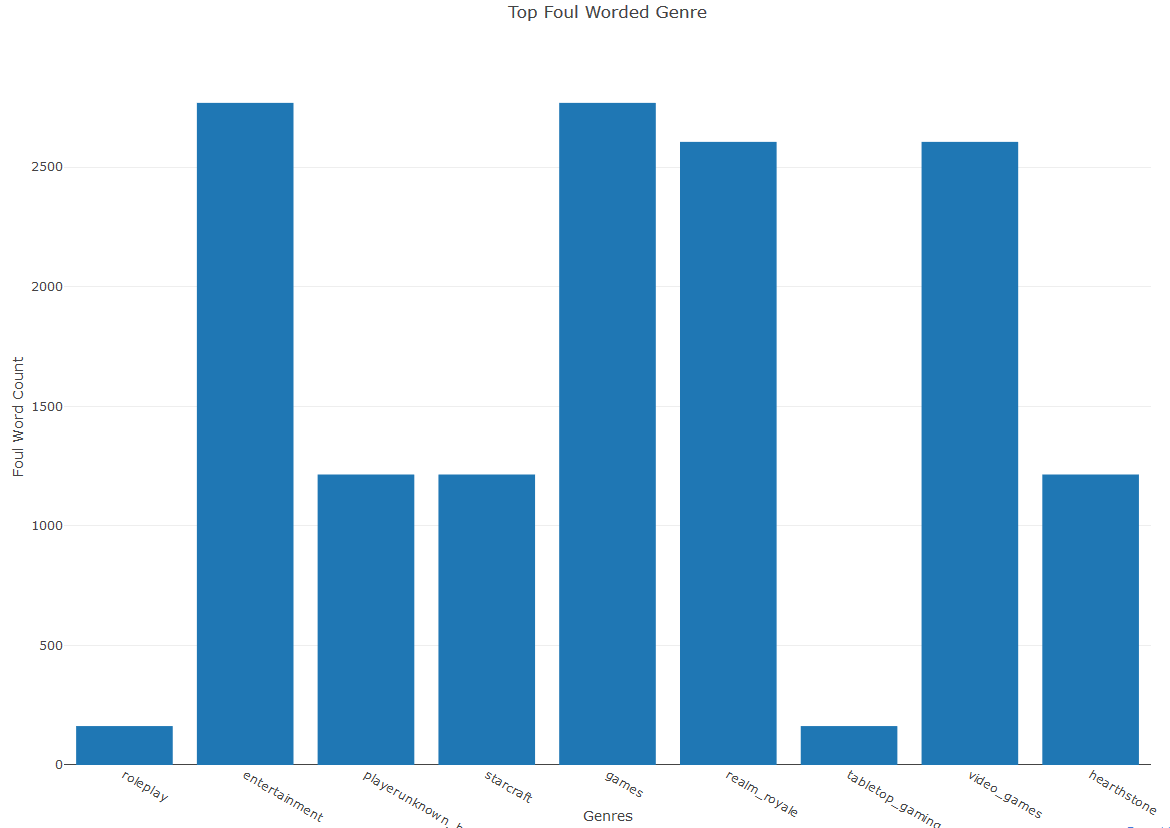
\includegraphics[height=4cm,keepaspectratio]{FoulWordGenres.png}
    \captionsetup                               {justification=centering}
    \caption                                    {Genres Foul Word Usage}
    \label                                      {fig:FoulWordGenres}
\end{figure}

\begin{figure}[h]
    \centering
    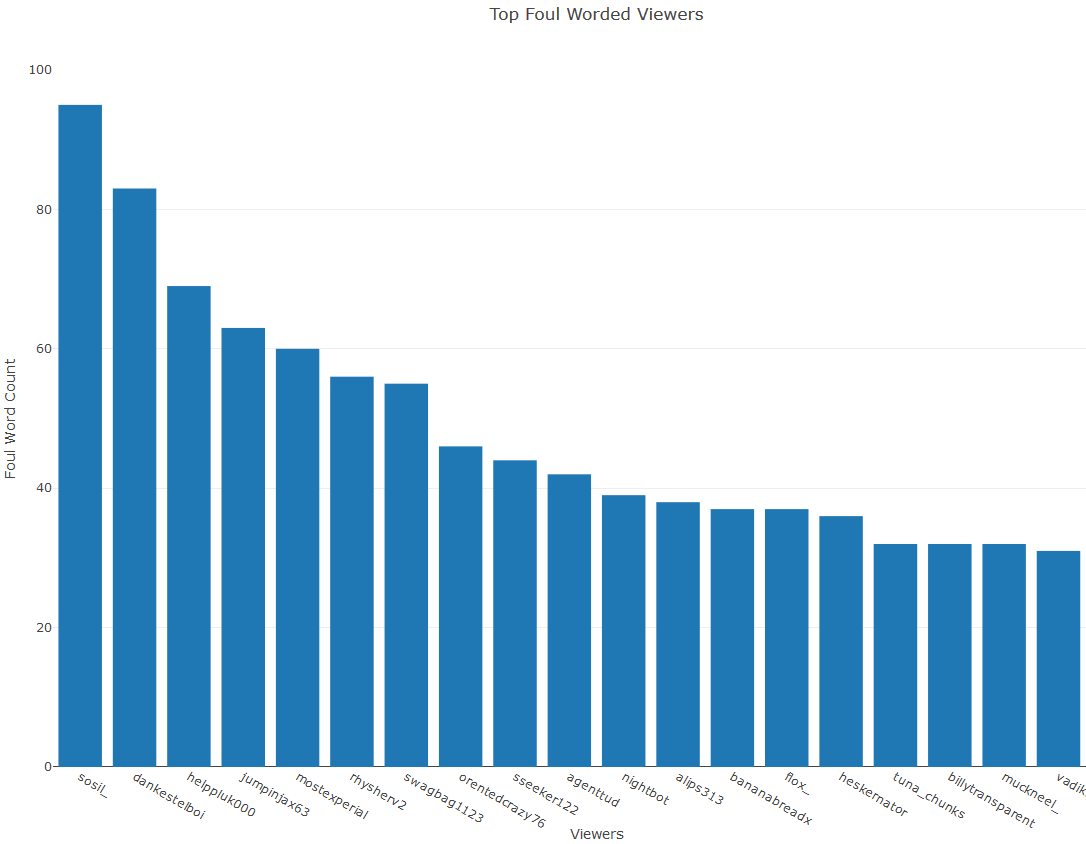
\includegraphics[height=4cm,keepaspectratio]{FoulWordViewersRank.png}
    \captionsetup                               {justification=centering}
    \caption                                    {Viewers Ranked by Foul Word Usage}
    \label                                      {fig:FoulWordViewersRank}
\end{figure}

\clearpage

\begin{figure}[h]
    \centering
    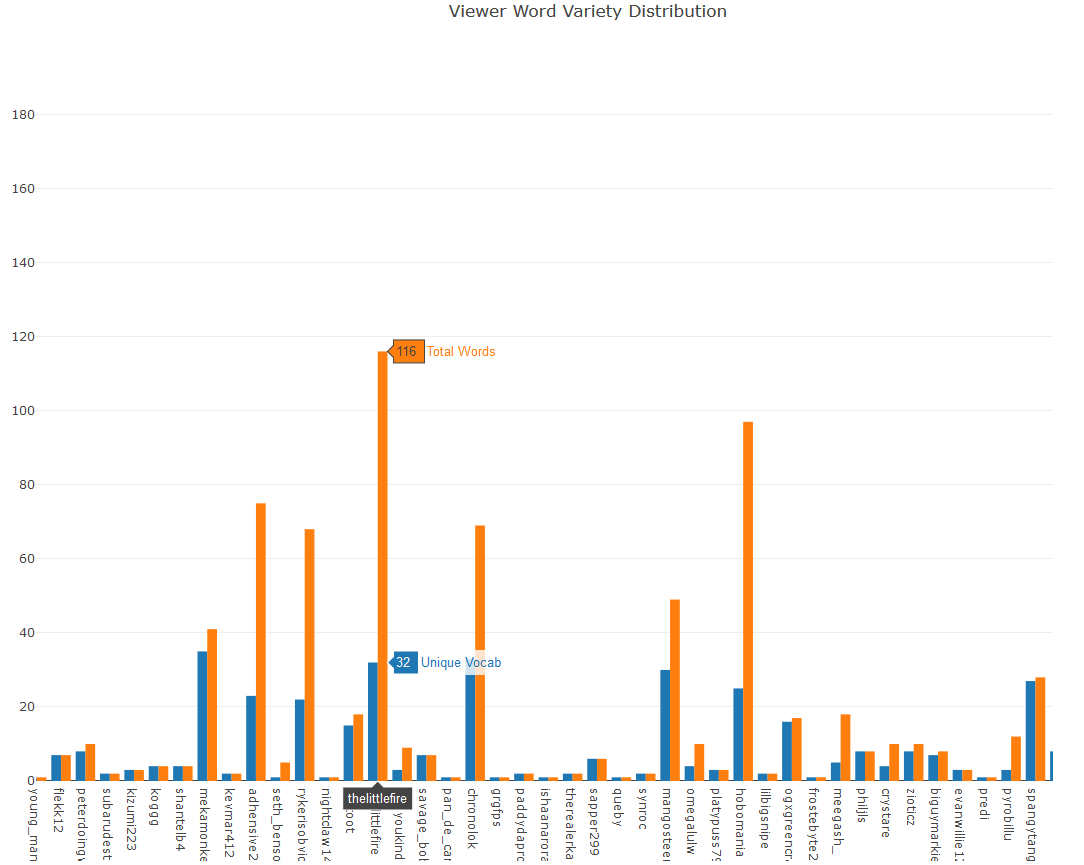
\includegraphics[height=4cm,keepaspectratio]{ViewersWordUsage.png}
    \captionsetup                               {justification=centering}
    \caption                                    {Viewers Word Usage \\
                                                 Blue: Unique Vocabulary \\
                                                 Orange: Total Word Utterances}
    \label                                      {fig:ViewersWordUsage}
\end{figure}

\subsection{Limitations and Future Improvements}
After both milestone runs, a number of potential improvements were noted, allowing room for future possible work on the proposed infrastructure to be carried out.

\begin{itemize}
    \item The system security aspect was considered as beyond the scope of this project and thus was given little importance. Improvements include:
        \begin{itemize}
            \item Authentication hardening
            \item Creation of Linux users with limited privileges for the execution of all the involved OS processes.
        \end{itemize}
    \item All producers and consumers share the same Google account. Potential distribution between several Google accounts would aid in circumventing the limitations imposed by the platform \cite{GoogleSpeechQuotas} and thus improve the overall video processing performance.
    \item Improving system robustness by adding a watchdog VM, capable of monitoring external nodes and re-initiating those nodes which exit in an unhandled manner.
    \item Bash script automation could benefit from more robust user input validation.
    \item Better VM specification allocation, by testing and evaluating performance on better hardware allocation, through vertical scaling of VMs.
    \item Storm main memory consumption was noted to be gradually increase in terms of overall usage. This could be due to a potential memory leak on the Spout/Bolt logic.
\end{itemize}

\section{Conclusion}
In this report, the well established challenges of big data concerning aspects of a variety and a velocity nature, were addressed by a real time video and text processing system. The proposed architecture was broken down into a number of components, for which each individual usage and performance was evaluated through extracted metrics pertaining to two separate testing scenarios. The acquired data streams were stored inside of a graph warehouse, making retrieval and representation of word usage per viewer/streamer a possibility, facilitating any data mining and data extraction attempts from the acquired data.

\bibliographystyle{IEEEtran}  
\bibliography{BigDataReport}

\end{document}
